
\label{chap: methods}
In this section, two methods are presented that attempt to reduce the bias seen in the estimates from \cite{michelot_langevin_2019}. The first of these methods applies the Extended Kalman filter to an increased state-space model. The second is based on increasing the state space of the Langevin model using hidden states, then using the Monte Carlo method to integrate out the hidden states. 

\section{Extended Kalman Filter}
\parencite{kulikov_extended_2024} describes one method that tries to more accurately approximate the likelihood of diffusion processes using the extended Kalman filter. If we use the Euler-Maruyama method to describe a state-space model, we can then find a likelihood using the extended Kalman filter. In addition, we can improve this likelihood approximation by adding extra hidden states between the states that we have observed. For the Langevin process, the state space representation is 

$$\textbf{X}_{k+1} = f(\textbf{X}_k) + \textbf{w}_k = \textbf{X}_k + \frac{\gamma^2\Delta_k}{2}\nabla log(\pi(\textbf{X}_k)) + \textbf{w}_k$$

$$\textbf{Z}_k = h(\textbf{X}_k) + \textbf{w}_k$$

where $\textbf{w}_k$ has a gaussian distribution with $0$ mean and covariance $\gamma^2\Delta_k I_{2*2}$, and $\textbf{v}_k$ has $0$ mean and covariance $\textbf{R}$. In the case where the process is being observed directly, the function $h$ is the identity function, and the matrix $\textbf{R}$ is a zero matrix. The method described in \parencite{kulikov_extended_2024} adds a mesh of $L$ hidden states to the state-space model between observations $\textbf{Z}_i$ and $\textbf{Z}_{i+1}$. When using the extended Kalman filter on the added mesh states, only the predict step is performed since there are no observations. The likelihood is then computed using \eqref{eq: EKF likelihood}, which can be used to make estimates of the parameters. 

\

The matrices $\textbf{F}_k$ and $\textbf{H}_k$ in Section~\ref{sec: EKF} are the Jacobians of the transition and observation functions. Since the observation function $h$ is the identity function, we get $H_k = I_{2*2}$. Furthermore, we have $\textbf{F}_k = Jac(f) = Jac(\textbf{x} + \frac{\gamma^2 \Delta}{2}\nabla log(\pi(\textbf{x}))) = I_{2*2} + \frac{\gamma^2 \Delta}{2} H(\log(\pi(\textbf{x})))$. $H(\log(\pi(\textbf{x})))$ is the Hessian of the log of the utilization distribution, which, if we insert the resource selection function, becomes $H(\sum_{i=1}^n \beta_i c_i(\textbf{x})) = \sum_{i=1}^n \beta_iH( c_i)(\textbf{x})$. The calculation of this matrix involves taking the second derivative of the covariate functions. This can be found using the method described in Subsection~\ref{subsec: second derivative}.


\begin{comment}
    
ADD THIS TO THE DISCUSSION
{
When using the extended Kalman filter on the added mesh-nodes, only the predict step i performed. For the predicted state estimate, this means that the prediction of the following state is made using a deterministic path following the gradient of the UD. If $x_l$ are the mesh states, then $x_1 = X_{k-1|k-1}$, $x_{l+1} = x_l + \frac{\gamma^2\Delta}{2(L+1)} \nabla log(\pi(x_l))$ for $l = 2, \dots, L$, until we find the predicted state estimate $\hat{X}_{k|k-1} = x_L + \frac{\gamma^2\Delta}{2(L+1)} \nabla log(\pi(x_L))$. For the predicted estimate covariance we get $p_1 = P_{k|k-1}$, $p_l = F_l p_{l-1} F_l + Q$ for $l=2, \dots, L$ and $P_{k+1|k} = p_l$. Where $p_l$ is the mesh state covariances, $F_l$ is the Jacobian of the transition function evaluated at the mesh states.

\

To demonstrate how the estimate of the extended Kalman filter works in practice, we can take two points of the simulated Langevin process, and use the EKF to find an estimate for the second state using the first. We can then make a 90\% confidence interval for each state estimate by using $x±z_{\alpha/2}\sqrt{var}
$ with $\alpha = 0.9$.

\


\begin{figure}[H]
    \centering
    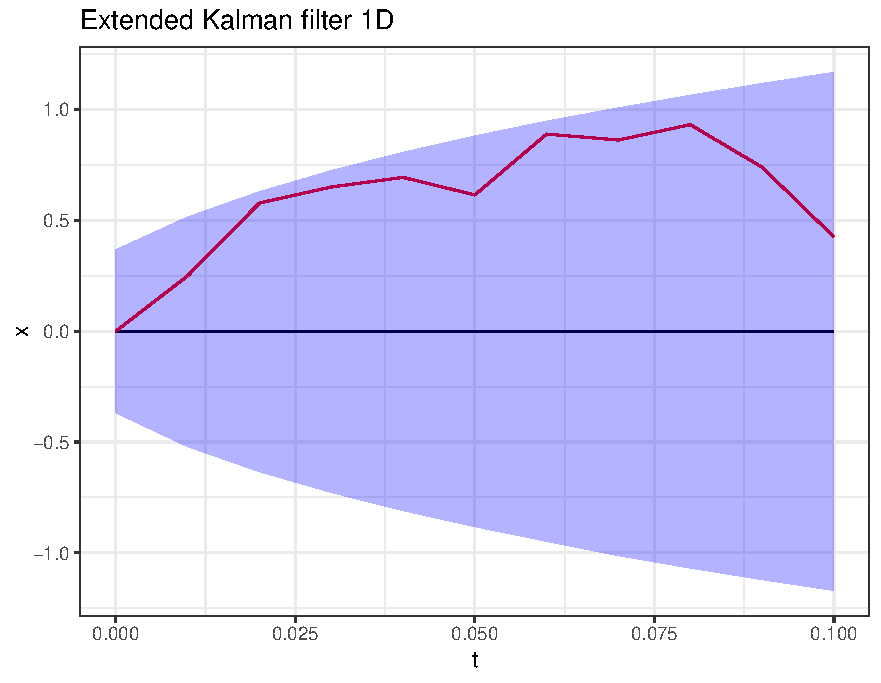
\includegraphics[width=\linewidth]{Images/ch3/EKF figure 1D.pdf}
    \caption[Extended Kalman filter]{Plot of extended Kalman filter state estimates. The black line shows the predicted state estimates over a time grid from 0 to 0.1, with increments 0.01. The blue ribbon shows the 90\% confidence interval for the predicted state estimate, and the red line show the Langevin process that is being estimated. The parameters used for generating the Langevin process and the EKF path are the same}
    \label{fig:EKF 1D}
\end{figure}

\


Figure Figure~\ref{fig:EKF 1D} demonstrates an issue with the extended Kalman filter. The figure shows very little movement in the predicted state estimates (black) compared to the Langevin process (red). This is partly due to the example used. In the example the diffusion of the Langevin process dominates, and the drift from the covariates plays a much smaller role. In the setting of animal movement this is appropriate because the movement is highly unpredictable, but when using the EKF it means that the predicted state estimates don't approximate the Langevin process well. 

\

The predicted estimate covariance is partly based on the previous predicted state estimate, so an issue that comes up when the predicted estimate covariance moves differently from the Langevin process is that the predicted estimate covariance is also affected. Normally the EKF is used only on states where we have observations. The problem with increasing deviation from the real process does not occur in this case. In contrast when adding extra hidden states, the error in predicting one state is passed on to the next state. Despite this, the covariance estimate in figure~\ref{fig:EKF 1D} shows that the simulated Langevin process is within the 90\% confidence interval. 

\

As mentioned earlier, in the case used in figure~\ref{fig:EKF 1D}, the diffusion dominates the drift becasue of high diffusion constant used compared to the gradient of the covariates. We can test a case where the diffusion constant $\gamma$ is much smaller, and the value $\beta \gamma^2$ is kept as the same used in figure~\ref{fig:EKF 1D}. We should then expect the estimated path using the predict step of the EKF to be similar to the simulated Langevin process. The information which used to compute the estimate covariance $P_l$ using the jacobian of the transition function should also be more correct in this case.

\begin{figure}[H]
    \centering
    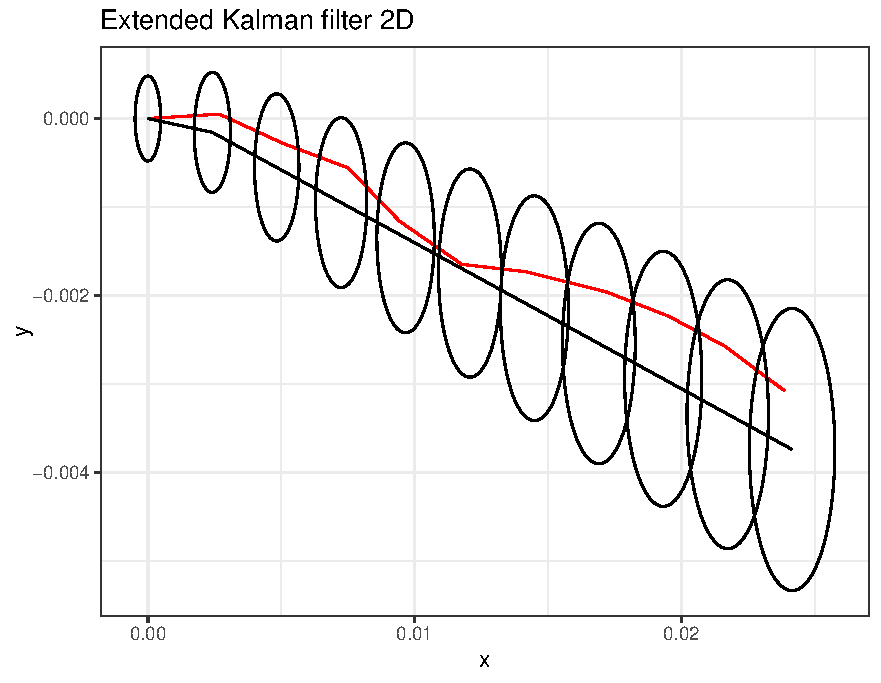
\includegraphics[width=\linewidth]{Images/ch3/EKF path 2D.pdf}
    \caption[Extended Kalman filter]{Plot of extended Kalman filter state estimates. The black line shows the predicted state estimates over a time grid from 0 to 0.1, with increments 0.01. The elipses show the evolving 90\% confidence levels set computed using the predicted estimate covariance, and the red line show the Langevin process that is beeing estimated. The parameters used are the same for the Langevin process and the EKF}
    \label{fig:EKF 2D}
\end{figure}
THIS FIGURE HAS TO SMALL TIME INTERVAL. THE INTERVALS SHOULD BE STRIPED

\

Figure~\ref{fig:EKF 2D} shows that when the diffusion of the Langevin process is small compared to the drift, the extended Kalman filter estimates the unobserved states of the process well. 




This example is not suited for animal prediction, since animal movements are highly random, and would have a large diffusion constant compared to 

In multiple dimension the EKF might perform worse since there is more chaos?
curse of dimmensionality


}

%Discussion: There is no guarantee that the extended Kalman filter will converge to the correct likelihood.

\end{comment}







\section{Monte-Carlo Estimation of Likelihood}
\label{sec: Monte Carlo Estimation}
For the second method, consider a hidden variable $\textbf{Z} = (\textbf{Z}_1, \dots \textbf{Z}_n)$ that is a set of states between two observations of the Langevin process $\textbf{X}_k$ and $\textbf{X}_{k+1}$. We can write the joint density of transitioning from the first observation to the second observation via these states as 

$$p(\textbf{X}_{k+1}, \textbf{Z} | \textbf{X}_k) = p(\textbf{X}_{k+1}|\textbf{Z})p(\textbf{Z}|\textbf{X}_k) = q_{\Delta_k/(N+1)}(\textbf{X}_{k+1}|\textbf{Z}_N)\dots q_{\Delta_k/(N+1)}(\textbf{Z}_1|\textbf{X}_k)$$ 

From here we can integrate out the hidden variable to get the likelihood of the observations, 


$$p(\textbf{X}_{k+1}|\textbf{X}_k) = \int q_{\Delta_k/(N+1)}(\textbf{X}_{k+1}|\textbf{Z}_N)\dots q_{\Delta_k/(N+1)}(\textbf{Z}_1|\textbf{X}_k)d\textbf{Z}$$

Because the time difference between the states in $\textbf{z}$, is smaller than the time difference between $\textbf{X}_{k+1}$ and $\textbf{X}_k$, so $q_{\Delta_k/(N+1)}$ should be a better approximation for the Langevin process than $q_{\Delta_k}$. We can approximate this integral by using the Monte Carlo method described in Subsection~\ref{sec: Monte Carlo integration}. We can sample M paths $\textbf{Z}^i = (\textbf{Z}_1^i, \dots,\textbf{Z}_N^i)$ each with N nodes, using $\textbf{Z}_{j+1}^i = \textbf{Z}_j^i + \nabla log(\pi(\textbf{Z}_j^i)) + \frac{\Delta_k\gamma^2}{N+1}\bm \epsilon_j^i$ where $\bm \epsilon_j^i$ standard two-dimensional Gaussian distributions for $i=1, \dots , M$ and $j = 1,\dots , N$, using $\textbf{Z}_0^i = \textbf{X}_k$. We then get the likelihood estimate

$$
\hat{L}(\bm \beta , \gamma^2|X_k, X_{k+1}) =  \frac{1}{M}\sum_{i=1}^M q_{\Delta_k/(N+1)}(\textbf{X}_{k+1}|\textbf{Z}^i_N)\dots q_{\Delta_k/(N+1)}(\textbf{Z}^i_1|\textbf{X}_k)
\label{eq: montecarlo likelihood}
$$

If the hidden states $\textbf{Z}_i$ are evenly distributed in time, and the number of states $N$ is sufficiently high, then they should accurately approximate the Langevin process, as evidenced in figure~\ref{fig:MALA}. In turn, this means the Monte Carlo likelihood estimate should be unbiased for the transition likelihood of the Langevin process. An important point about this likelihood estimate is that it is stochastic, which has to be taken into account when doing estimation. 

\begin{comment}
\parencite{durham_numerical_2002} uses the Nelder-Mead optimization algorithm to find maximum likelihood estimates. This is a direct search method, meaning it does not compute the gradient of the function that is being minimized. This is an advantage when the likelihood estimate is stochastic since gradients require evaluating the function at close intervals which may be subject to a lot of noise.     
\end{comment}


\

\subsection{Importance Sampling}
\label{subsec: importance sampling}
One problem with the likelihood estimator \eqref{eq: montecarlo likelihood} is that the last step of the probability $q_{\Delta_k/(N+1)}(\textbf{X}_{k+1}|\textbf{Z}_N)$ often has a small value. This is because the paths $\textbf{Z}$ diverge more and more from the true path that the Langevin process used, which means that for many paths the last state ends far away from the next observation. In turn, this means that most simulations of $\textbf{z}$ contribute very little to the estimated likelihood. And a small number of simulations that end up landing close to $X_{k+1}$ end up contributing to a large part of the estimate, giving the estimate high variance. \parencite{durham_numerical_2002} improves upon the Monte-Carlo estimate of the transition by using importance sampling, described in Subsection~\ref{subsec: importance sampling}, into the method. Instead of sampling $\textbf{Z}$ from the Langevin process, they sample it from a different distribution $p$ and use the estimate

\begin{equation}
\hat{L}(\theta|X_k, X_{k+1}) = \frac{1}{M}\sum_{i=1}^M \frac{q_{\Delta_k/(N+1)}(\textbf{X}_{k+1}|\textbf{Z}^i_N)\dots q_{\Delta_k/(N+1)}(\textbf{Z}^i_1|\textbf{X}_k)}{p(\textbf{Z}_i)}
\label{eq: importance sampling likelihood}
\end{equation}


\parencite{durham_numerical_2002} proposes a Brownian bridge between the observations $\textbf{X}_k$ and $\textbf{X}_{k+1}$ for the distribution $p$. This is a simulation of a Brownian motion $\gamma \textbf{B}_t$, conditioned on having endpoints $\textbf{X}_k$ and $\textbf{X}_{k+1}$. A Brownian bridge variable $\textbf{B}_l$ can be simulated as a multivariate Gaussian distribution with mean $\bm \mu_l = \textbf{X}_k + l(\textbf{X}_{k+1}-\textbf{X}_k)/N$ and covariance matrix $\bm \Sigma$ with $\bm \Sigma_{ij} = \bm \Sigma_{ji}= \Delta \gamma^2(1-\frac{i}{N+1}) \frac{j}{N+1}$ for $i = 1, \dots , N$ and $j = 1, \dots, i$. Where N is the number of mesh nodes in the bridge. We can write the full log-likelihood as 


$$
\hat{l}(\bm \beta, \gamma^2) = \sum_{i = 1}^K log( \frac{1}{M}\sum_{j=1}^M \frac{1}{P_{ij}}\prod_{k=0}^N \mathcal{N}(B_{ijk+1} ; B_{ijk+1} - \frac{\Delta \gamma^2}{2}, \Delta\gamma^2 I_{2*2}))
$$

where the first and last elements of the bridges $B_{ij0}$ and $B_{ijN+1}$ are the observed values of the Langevin process $X_i$ and $X_{i+1}$ respectively, and $P_{ij}$ is the density of the j-th bridge between $\textbf{X}_{i+1}$ and $\textbf{X}_i$.

To demonstrate how the Brownian bridges reduce variance we can take two points of the simulated Langevin process, which has been thinned. We can then make a number of simulations of both the Langevin process and the Brownian bridge, using the same parameter for the Langevin process speed and the Brownian bridge variance.

\

\begin{figure}[H]%
    \centering
    \subfloat[\centering Langevin process simulations]{{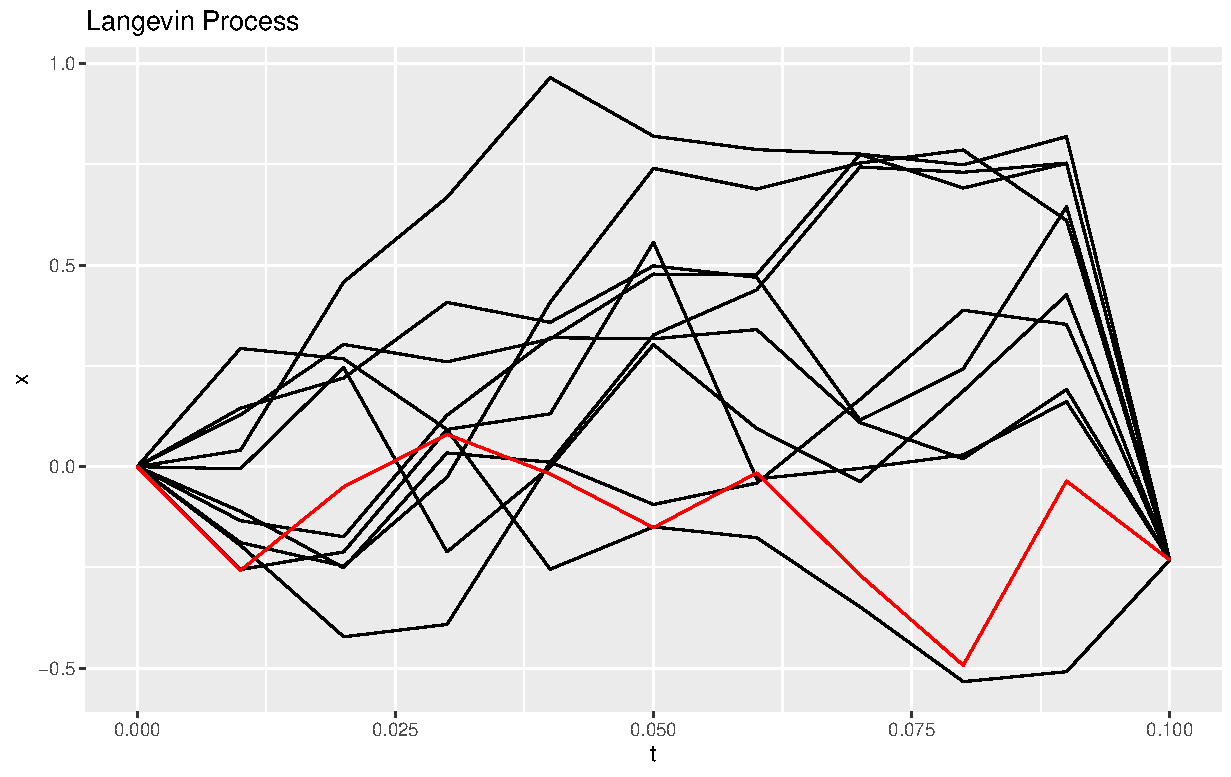
\includegraphics[width=\linewidth]{Images/ch3/Langevin process path figure.pdf} }}%
    \qquad
    \subfloat[\centering Brownian bridge simulations]{{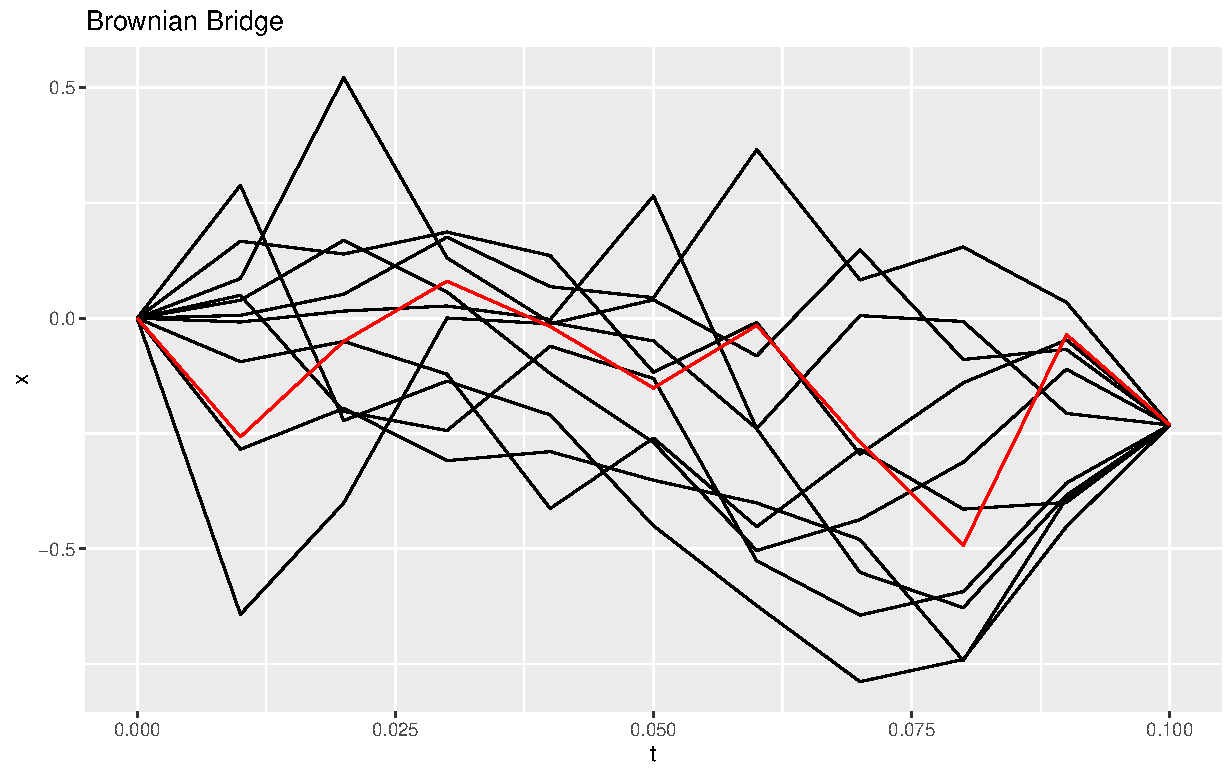
\includegraphics[width=\linewidth]{Images/ch3/Brownian bridge path figure.pdf} }}%
    \caption[Langevin and Brownian bridge paths]{(a): plot of one dimension of ten simulated Langevin process in black, with the true Langevin process that we want to estimate in red. the last step shows the path that would be needed to be taken to reach the last state of the Langevin process that we are estimating. (b): plot of ten simulations of Brownian bridges with endpoints at the end points of the Langevin process that we are estimating, shown in red.}%
    \label{fig:monte carlo paths}%
\end{figure}

\

Figure~\ref{fig:monte carlo paths} shows one dimension of the paths simulated from the Langevin process in (a) and the Brownian bridge in (b), plotted against time. The true path of the Langevin process, whose endpoints we are simulating based on, is shown in red. The first figure shows how the final step of the simulated Langevin processes (black), in many cases, deviates from the Langevin process that we are trying to estimate. Since there is high variability in the distance from the last point in $\textbf{Z}^i$ to the next observation, this can cause the likelihood estimate to have a high variance. The second plot, on the other hand, shows that the proposed paths do not include large jumps, as the first plot. Because of this, using the Brownian bridges as a proposal density might reduce the variance of the likelihood estimate. judging by the Langevin process in red, the Brownian bridges are also plausible transitions of the Langevin process. 

\

Using the theory of subsection~\ref{subsec: importance sampling theory}, the density of the variables being integrated with respect to $f(x)$, is the Euler Maruyama transition probability. The density of the proposal, $g(x)$, is the probability of the Brownian bridge, and the function we are integrating over$h(x)$, is the probability transitioning in the last step to the end points of the Langevin process $q_{\Delta_k/(N+1)}(\textbf{X}_{k+1}|\textbf{Z}_N)$. The support of $f$ is the same as the support of $g$, since both the Langevin process and the Brownian bridge can theoretically take on any value for any of the mesh states. When $g$ is small, $h$ is also likely to be small, indicating that the Brownian bridge should reduce the variance. \parencite{durham_numerical_2002}  shows that the importance sampling estimator reduces the root mean square error to the Langevin process, compared to using the Monte Carlo estimate.


\subsection{Pre-Computing Brownian Bridges}
\label{subsec: precomputing brownian bridges}
Even when using importance sampling, it can take a long time to compute the likelihood. A large portion of the computational complexity of the likelihood is simulating the Brownian bridges and computing the gradients of the covariates at the points of the bridges. A way to circumvent some of this computation would be to simulate the bridges and compute the gradients before evaluating the likelihood. This might save time in situations where we are evaluating the likelihood many times, like in numerical optimization. Pre-computing the Brownian bridges would necessitate having a value for the speed parameter beforehand. One way of doing this is to use the estimate from \parencite{michelot_langevin_2019} for the speed parameter. For large time differences between observations, this estimator underestimates the speed. However, if the variance used in the proposal has little effect on the likelihood estimate, this could still give the correct parameter estimates. 




\begin{comment}
    
\section{Assessing the Models}
\label{sec: assessing the models}
 In this chapter three likelihood approximations for the Langevin process likelihood have been explored. Method one being based on the use of the extended Kalman filter. method two approximates the likelihood by using Brownian bridges for importance sampling to integrate over intermediate states between observations. And method three pre-computes these bridges before evaluating the likelihood. To find maximum likelihood estimates for these likelihoods I use the "L-FBGS-B" method as implemented in the R packages "optim" and "optimParalell". For method two and three, I use an analytical gradient which is derived in appendix~\ref{Appendix C}. This gradient assumes that the proposal density remains constant when we take the derivatives. This is true for method three where we are using the same bridge each time we evaluate the likelihood. For method two however, this is not true since the bridges are simulated each time the likelihood is evaluated. I choose to use this gradient for both method 2 and 3 because the importance sampling estimate converges for any proposal distribution, so we can expect the changes in the likelihood approximation to be small, when the change in the variance parameter used in the proposal is small.

\

To assess the three methods, tracks were simulated from the Langevin process using the function "simLangevinMM" form the R package "Rhabit"\cite{michelot_langevin_2019} with a resolution of $\Delta t = 0.01$, using the perlin noise and euclidean norm displayed in figure~\ref{fig:covariate plots} as covariates. The tracks were then thinned to give appropriate resolutions for the observations of the process. the parameters used were $\gamma^2 = 5$ and $\beta=(4,2,-0.1)$.

\

To test method one, 100 tracks were simulated each with 5000 observations with a resolution of $\Delta t = 0.1$. For each track, the parameters $\gamma^2$ and $\beta$ were estimated using both method one and the estimator described in section~\ref{sec: estimating parameters}. The time resolution used in the extended Kalman filter in method one was the same as the thinning. From these estimates box-plots were made comparing the two methods for each of the parameters. The code used to implement this experiment can be found in the git hub repository in appendix~\ref{Appendix: github repo}

\

The same tests were done for method 2 and 3. The first of these was to test the performance of the methods at resolutions $\Delta t = \{0.1, \ 0.5, \ 1\}$ for the observations. 100 tracks were simulated for each of the resolutions, each containing 5000 observations. The parameters $\gamma^2$ and $\beta$ were then estimated, and the estimates were displayed in a box-plot, comparing the estimates for each of the parameters. The code implementing this experiment can be found in the git hub repository under the filename "varying thin estimates Brownian bridge likelihood.R" for method two and under "varying thin estimates precomputed Brownian bridge likelihood.R" for method three.

\

The second test made to method method two and three, was to test the effect of the number of path nodes $N$ on their performance. 100 tracks were simulated, each containing 5000 observations, and having a resolution $\Delta t = 1$ between observations. The parameters $\gamma^2$ and $\beta$ were then estimated for $N = \{4, 9, 49, 99\}$ corresponding to resolutions $\Delta t = \{0.2, 0.1, 0.02, 0.01\}$ respectively. The estimates were then displayed using box-plots comparing the estimates for each of the parameters. The code used to generate the box-plot can be found in the git hub repository under the file name "varying N estimates Brownian bridge likelihood.R" for method 2 and "varying N estimates precomputed Brownian bridge likelihood.R" for method three.

\

For the third test, 100 tracks were simulated, each containing 5000 observations with a resolution of $\Delta t = 1$ between the observations. estimates were found for $\gamma^2$ and $\beta$ using these tracks for each of the values $M = \{5, 10, 50, 100, 200\}$. The estimates were then displayed in box-plots comparing the estimated for each of the parameters. The code for generating the box-plots can be found in the git hub repository under the file name "varying M estimates Brownian bridge likelihood.R" for method two, and under "varying M estimates precomputed Brownian bridge likelihood.R" for method three.


-  i am using rhabit to estimate the parameter for the precomputed bridges
- write about why i use L-BFGS-B
- have a separate experiment for time takes to do estimates and the variance of the estimators themselves
- The EKF experiment uses optimparalell
\end{comment}



\begin{comment}
\section{Including Observation Error}
The estimates found using the method in subsection~\ref{subsec: importance sampling} do not account for observation error in the track data. The estimator found by \cite{michelot_langevin_2019} does not account for observation error either. Instead they circumvent this error by preprocessing their data. They do this by using the package "Crawl" \cite{johnson2018crawl}, which finds estimates of the true postions of the observations using the Kalman filter. This method can also be used for the estimator found in subsection~\ref{subsec: importance sampling}. In this section i present an alternative to estimating the Langevin process parameter, whcich accounts for measurement error.

\

I will assume that the observation errors $\epsilon_k$ are i.i.d Gaussian distributed, with zero mean and covariance $r^2 I_{2*2}$. The process of observing the Langevin process can be expressed as a hidden variable model, where we have observations $y_k$ and the hidden process $x_k$. Because all the information about the observations $y_k$ is held in the hidden variable $x_k$ we can write
$$
p(y_{k+1}, x_{k+1}|y_k,x_k) = p(y_{k+1},x_{k+1}|x_k) = p(y_{k+1}|x_{k+1})p(x_{k+1}|x_k)
$$

We can find the density of $y_{k+1}$ conditional on $x_k$ by integrating out $X_{k+1}$

$$
p(y_{k+1}|x_k) = \int p(y_{k+1}, x_{k+1}|x_k) dx_{k+1} = \int p(y_{k+1}|x_{k+1})p(x_{k+1}|x_k) dx_{k+1}
$$

Since the observation density is symmetric, we can integrate out $x_k$ to find the density of $y_{k+1}$ conditioned on $y_k$

$$
p(y_{k+1}|y_k) = \int p(y_{k+1},x_k|y_k) dx_k = \int p(y_{k+1}|x_k)p(x_k|y_k) dx_k
$$

We can then combine the three formulas above to get 

$$
p(y_2|y_1) = \int \int p(y_{k+1}|x_{k+1})p(x_{k+1}|x_x)p(x_k|y_k) dx_k dx_{k+1}
$$

The density Langevin transition density $p(x_{k+1}|x_k)$ is difficult to estimate, as has been discussed in earlier sections. To correct for this i will do as in section subsection~\ref{subsec: Monte-Carlo Estimation}, and add a series of intermediate hidden variable $\textbf{z}$ in between $x_k$ and $x_{k+1}$. 

$$
p(y_{k+1}|y_k) = \int \int p(y_{k+1}|x_{k+1})p(x_{k+1}|\textbf{z})p(\textbf{z}|x_k)p(x_k|y_k) dx_k \textbf{z} dx_{k+1}
$$

From here we can use the importance sampling estimator used in subsection~\ref{subsec: importance sampling}, but instead of using Brownian brdiges between observations, we use Brownian bridges between points simulated observation error around the observed locations. These points are simulated according to the observation model, which in our case is a normal distribution with zero mean and variance $r^2$  

$$
\hat{l}(\beta, \gamma^2) = \sum_{i = 1}^K log( \frac{1}{M}\sum_{j=1}^M \frac{1}{P_{ij}}\prod_{k=0}^N \mathcal{N}(B_{ijk+1} ; B_{ijk+1} - \frac{\Delta \gamma^2}{2}, \Delta\gamma^2 I_{2*2}))
$$

Where $B_{ij0}$ is the j-th point simulated around observation i, and $B_{ijN}$ is the j-th point simulated around observation i+1.



$$
\hat{l}(\beta, \gamma^2) = \sum_{i = 1}^K log( \frac{1}{M}\sum_{j=1}^M P_{ij}  p(\sqrt{\Delta}\gamma z_{ij1} + \mu_{ij1}; X_i + r^2\epsilon_{ij} ) p(X_{i+1} + r^2\epsilon_{i+1j} | \sqrt{\Delta}\gamma z_{ij1} + \mu_{ij1})\prod_{k=1}^{N-1}(\sqrt{\Delta}\gamma z_{ijk+1}  + \mu_{ijk+1}; \sqrt{\Delta}\gamma z_{ijk}  + \mu_{ijk}))
$$

$\mu_{ijk}$ is the k-th interpolated value between $X_i + r^2\epsilon_{ij}$ and $X_{i+1} + r^2\epsilon_{i+1j}$, $p(y|x) = \mathcal{N}(y; x + \frac{\Delta \gamma^2}{2}g(x)\beta$ where $g$ is the a matrix with ncov number of columns and two rows, which is the set of gradients of ncov spatial covariates
\end{comment}














